
%(BEGIN_QUESTION)
% Copyright 2009, Tony R. Kuphaldt, released under the Creative Commons Attribution License (v 1.0)
% This means you may do almost anything with this work of mine, so long as you give me proper credit

Sketch connecting wires such that the relay will energize and turn the lamp {\it off} when the normally-open (NO) pushbutton switch is pressed (i.e. the lamp should be {\it on} when the pushbutton switch is not being pressed).  Be sure to wire the relay in such a way that current (conventional flow) follows the directions indicated by the arrows, and that the switch only carries relay coil current (no lamp current in addition to coil current):

$$\includegraphics[width=15.5cm]{i03832x01.eps}$$

\underbar{file i03832}
%(END_QUESTION)





%(BEGIN_ANSWER)

Bear in mind that this is not the {\it only} possible circuit solution:

$$\includegraphics[width=15.5cm]{i03832x02.eps}$$

Challenge yourself by designing a different circuit to meet the same criteria! 

%(END_ANSWER)





%(BEGIN_NOTES)

%INDEX% Pictorial circuit review (relay circuit)

%(END_NOTES)


